\documentclass[conference,compsoc]{IEEEtran}
\usepackage{listings}
\usepackage{xcolor}
\usepackage{graphicx}
\usepackage{subfig}
\usepackage{amsmath}
\usepackage{amssymb}

\definecolor{codegreen}{rgb}{0,0.6,0}
\definecolor{codegray}{rgb}{0.5,0.5,0.5}
\definecolor{codepurple}{rgb}{0.58,0,0.82}
\definecolor{backcolour}{rgb}{0.95,0.95,0.92}

\lstdefinestyle{mystyle}{
    backgroundcolor=\color{backcolour},   
    commentstyle=\color{codegreen},
    keywordstyle=\color{magenta},
    numberstyle=\tiny\color{codegray},
    stringstyle=\color{codepurple},
    basicstyle=\ttfamily\footnotesize,
    breakatwhitespace=false,         
    breaklines=true,                 
    captionpos=b,                    
    keepspaces=true,                 
    numbers=left,                    
    numbersep=5pt,                  
    showspaces=false,                
    showstringspaces=false,
    showtabs=false,                  
    tabsize=2
}

\lstset{style=mystyle}

% *** CITATION PACKAGES ***
%
\ifCLASSOPTIONcompsoc
  % IEEE Computer Society needs nocompress option
  % requires cite.sty v4.0 or later (November 2003)
  \usepackage[nocompress]{cite}
\else
  % normal IEEE
  \usepackage{cite}
\fi

% correct bad hyphenation here
\hyphenation{op-tical net-works semi-conduc-tor}


\begin{document}
%
% Title
\title{Flow field through a porous media\\
GROUP NAME AND NUMBER}


% names and affiliations
\author{\IEEEauthorblockN{Name surname}
\IEEEauthorblockA{Student id\\dept./bsc course\\
email}
\and
\IEEEauthorblockN{Name surname}
\IEEEauthorblockA{Student id\\dept./bsc course\\
email}
\and
\IEEEauthorblockN{Name surname}
\IEEEauthorblockA{Student id\\dept./bsc course\\
email}}


% make the title area
\maketitle
\thispagestyle{plain}
\pagestyle{plain}

% As a general rule, do not put math, special symbols or citations
% in the abstract
\begin{abstract}
Optional. Short summary of the work - Max 120 words.
\end{abstract}

% no keywords




\section{Introduction}
% no \IEEEPARstart
Brief explanation of the overall assignment, of the performance reached, and of the components done.

\section{Part 1 - Theoretical aspects}

\subsection*{A -- Physics of the Problem}

\subsubsection{Dimensional Analysis and Scaling}

The problem involves predicting the transversal flow rate field $q(x_i,y_j)\ [\mathrm{m\,s^{-1}}]$ over a $32\times64$ grid from a binary cross-section image and four physical parameters. All quantities with their SI units are:
\begin{itemize}
  \item Pressure drop: $\Delta P\ [\mathrm{Pa}]$
  \item Channel length: $L\ [\mathrm{m}]$
  \item Fluid viscosity: $\mu\ [\mathrm{Pa\cdot s}]$
  \item Pixel area: $\Delta A = \Delta x\,\Delta y\ [\mathrm{m^2}]$
  \item Flow rate field output: $q(x,y)\ [\mathrm{m\,s^{-1}}]$
  \item Total flow: $Q = \sum_{ij}q(x_i,y_j)\,\Delta A\ [\mathrm{m^3\,s^{-1}}]$
\end{itemize}
The binary image $I(x_i,y_j)\in\{0,1\}$ is dimensionless. A unique velocity scale is formed from the four physical parameters by dimensional analysis:
\begin{equation}
  v_0 = \frac{\Delta P\,\Delta A}{\mu\, L}
  \quad\left[\frac{\mathrm{Pa}\cdot\mathrm{m}^2}{\mathrm{Pa\cdot s}\cdot\mathrm{m}}\right]
  = \left[\mathrm{m\,s^{-1}}\right].
  \label{eq:v0}
\end{equation}
This is the only independent velocity scale constructible from $(\Delta P, L, \mu, \Delta A)$; any other dimensional combination is a power of $v_0$.

\paragraph{Dimensionless learning problem.}
Normalizing $q$ by $v_0$ yields a dimensionless output $\tilde{q}$:
\begin{equation}
  \tilde{q}(x,y) = \frac{q(x,y)}{v_0}
                 = \frac{q(x,y)\,\mu\, L}{\Delta P\,\Delta A},
  \label{eq:dimless}
\end{equation}
so the learning problem reduces to
\begin{equation}
  \tilde{q} = \tilde{F}(I),
  \label{eq:dimless-problem}
\end{equation}
where $\tilde{F}$ maps a dimensionless binary image to a dimensionless field. All four physical parameters collapse into the single prefactor $v_0$.

\paragraph{Degree-1 homogeneous (scaling) form.}
A function $f$ is called a \emph{scaling} (degree-1 homogeneous) function if
\begin{equation}
  f(\lambda x_1,\dots,\lambda x_n) = \lambda\,f(x_1,\dots,x_n)
  \quad \forall\,\lambda > 0.
  \label{eq:homogeneous-def}
\end{equation}
Since $q$ is linear in $v_0$, the learning problem takes the scaling form
\begin{equation}
  q(x,y;\,\Delta P,L,\mu,\Delta A,I)
  = S\!\left(\frac{\Delta P\,\Delta A}{\mu L},\,I\right),
  \label{eq:scaling-form}
\end{equation}
where $S(\cdot)$ is a scaling function\footnote{$S(\cdot)$ here denotes the degree-1 homogeneous function in the sense of lecture notes Ch.~3. It is distinct from the hydraulic throughput scalar $S_h = \mu L Q/\Delta P\ [\mathrm{m}^4]$ introduced in Ch.~22 of the same notes.} satisfying $S(\lambda v_0,\,I) = \lambda\,S(v_0,\,I)$ for all $\lambda>0$. This encodes the physical law that doubling $v_0$ doubles the flow field everywhere.

\subsubsection{Symmetries of the Problem}

A symmetry of the learning problem is a transformation $T$ of the input image that induces a structured, predictable change in the output. Since $q(x,y)$ is a spatially distributed \emph{field}, the correct notion is \textbf{equivariance}: a model $f_\theta$ is equivariant under $T$ if
\begin{equation}
  f_\theta(T\cdot I)(x,y) = T\cdot f_\theta(I)(x,y).
  \label{eq:equivariance}
\end{equation}
This contrasts with \textbf{invariance}, which applies to scalar outputs that are \emph{unchanged} by $T$. The total flow $Q = \sum_{ij}q(x_i,y_j)\Delta A$ is invariant: $Q(T\cdot I) = Q(I)$.

The $32\times64$ rectangular domain admits the following three symmetries:

\begin{enumerate}
  \item \textbf{Left-right (horizontal) reflection} $T_\mathrm{LR}$: flipping $I$ about the vertical midplane yields a horizontally mirrored flow field, $q(T_\mathrm{LR}\cdot I)(x,y) = T_\mathrm{LR}\cdot q(I)(x,y)$.
  \item \textbf{Up-down (vertical) reflection} $T_\mathrm{UD}$: flipping $I$ about the horizontal midplane yields $q(T_\mathrm{UD}\cdot I)(x,y) = T_\mathrm{UD}\cdot q(I)(x,y)$.
  \item \textbf{180° rotation} $R_{180}$: rotating $I$ by $180°$ maps the rectangular domain onto itself, giving $q(R_{180}\cdot I)(x,y) = R_{180}\cdot q(I)(x,y)$.
\end{enumerate}

Note that $90°$ rotations are \emph{not} symmetries of this problem: a $90°$-rotated $32\times64$ image becomes a $64\times32$ image, which lies outside the input domain. The three transformations above generate the Klein four-group $\mathbb{Z}_2\times\mathbb{Z}_2$ of order 4 ($R_{180} = T_\mathrm{LR}\circ T_\mathrm{UD}$).

\subsubsection{Dataset Characterization}

The training set comprises $N=1500$ samples, each consisting of a $32\times64$ binary image $I$, a parameter tuple $(\Delta P, L, \mu, \Delta A)$, and the ground-truth flow field $q\in\mathbb{R}^{32\times64}$. Figure~\ref{fig:dataset-params} shows the marginal distributions of the four physical parameters. Figure~\ref{fig:dataset-examples} shows representative cross-sections alongside their flow rate fields. Figures~\ref{fig:flow-dist} and~\ref{fig:porosity} show the distributions of the flow rate field values and the open pixel fraction (porosity) across the training set.

\begin{figure}[h]
  \centering
  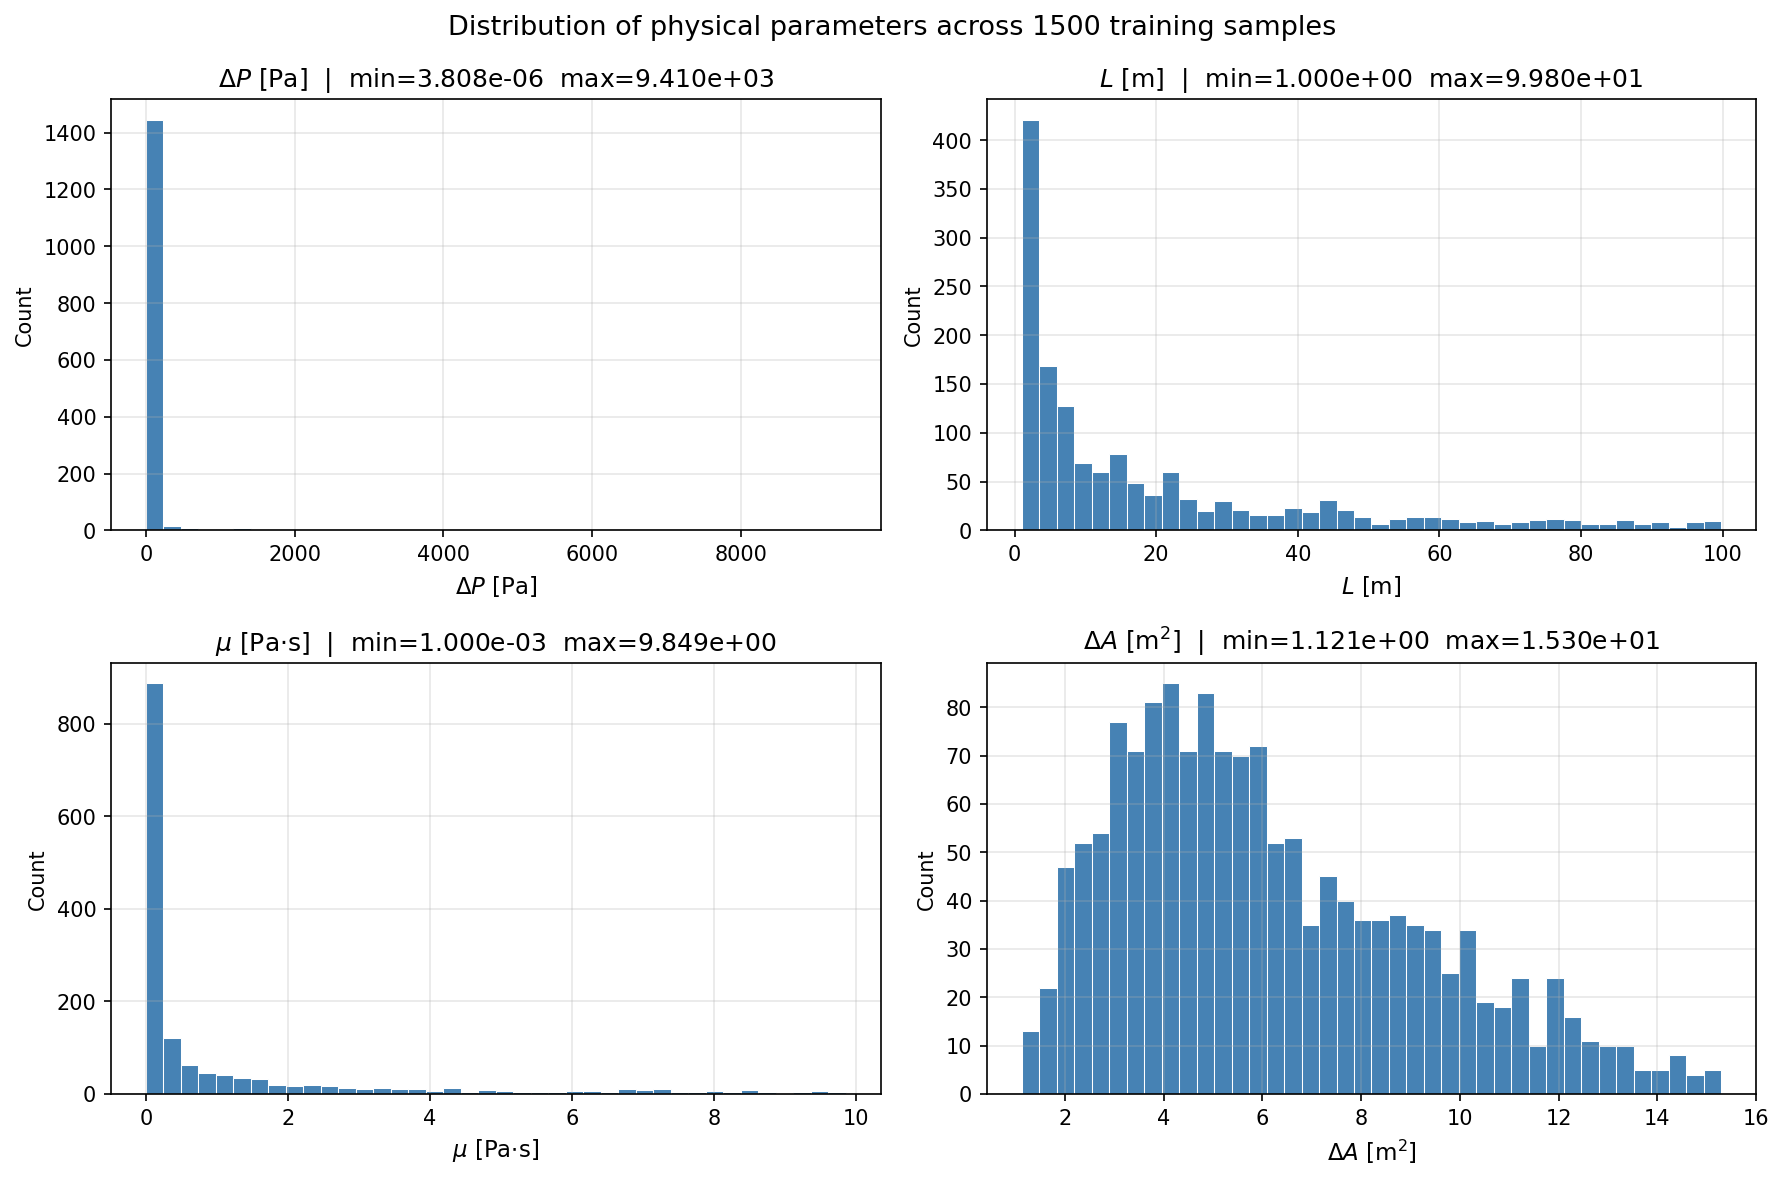
\includegraphics[width=\linewidth]{experiments/plots/exploration_parameter_distributions.png}
  \caption{Marginal distributions of $\Delta P\ [\mathrm{Pa}]$, $L\ [\mathrm{m}]$, $\mu\ [\mathrm{Pa\cdot s}]$, and $\Delta A\ [\mathrm{m^2}]$ over the 1500 training samples. Horizontal axis: parameter value; vertical axis: sample count.}
  \label{fig:dataset-params}
\end{figure}

\begin{figure}[h]
  \centering
  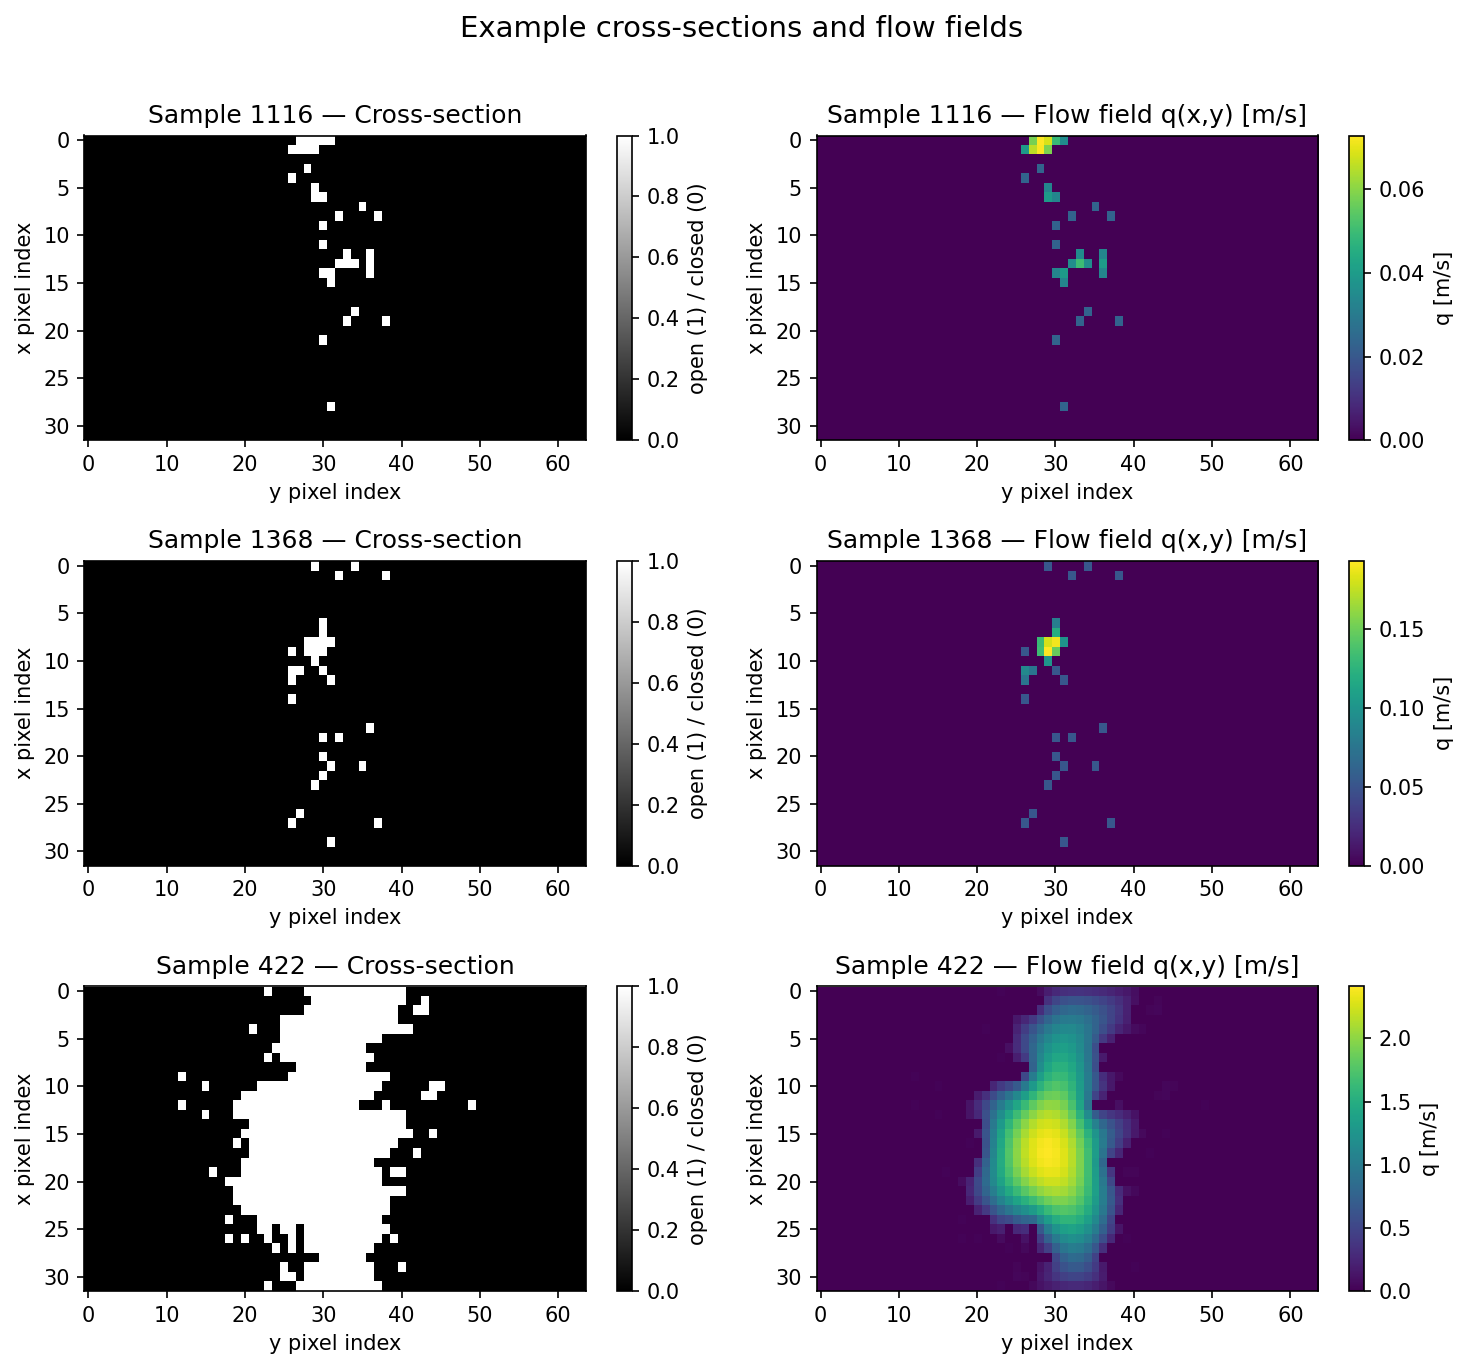
\includegraphics[width=\linewidth]{experiments/plots/exploration_cross_sections_and_flow.png}
  \caption{Representative training samples. Left column: binary cross-section images ($32\times64$ pixels; value 1 = open, 0 = closed). Right column: corresponding ground-truth flow rate fields $q(x,y)\ [\mathrm{m\,s^{-1}}]$. The flow is zero at all closed pixels — a hard physical constraint.}
  \label{fig:dataset-examples}
\end{figure}

\begin{figure}[h]
  \centering
  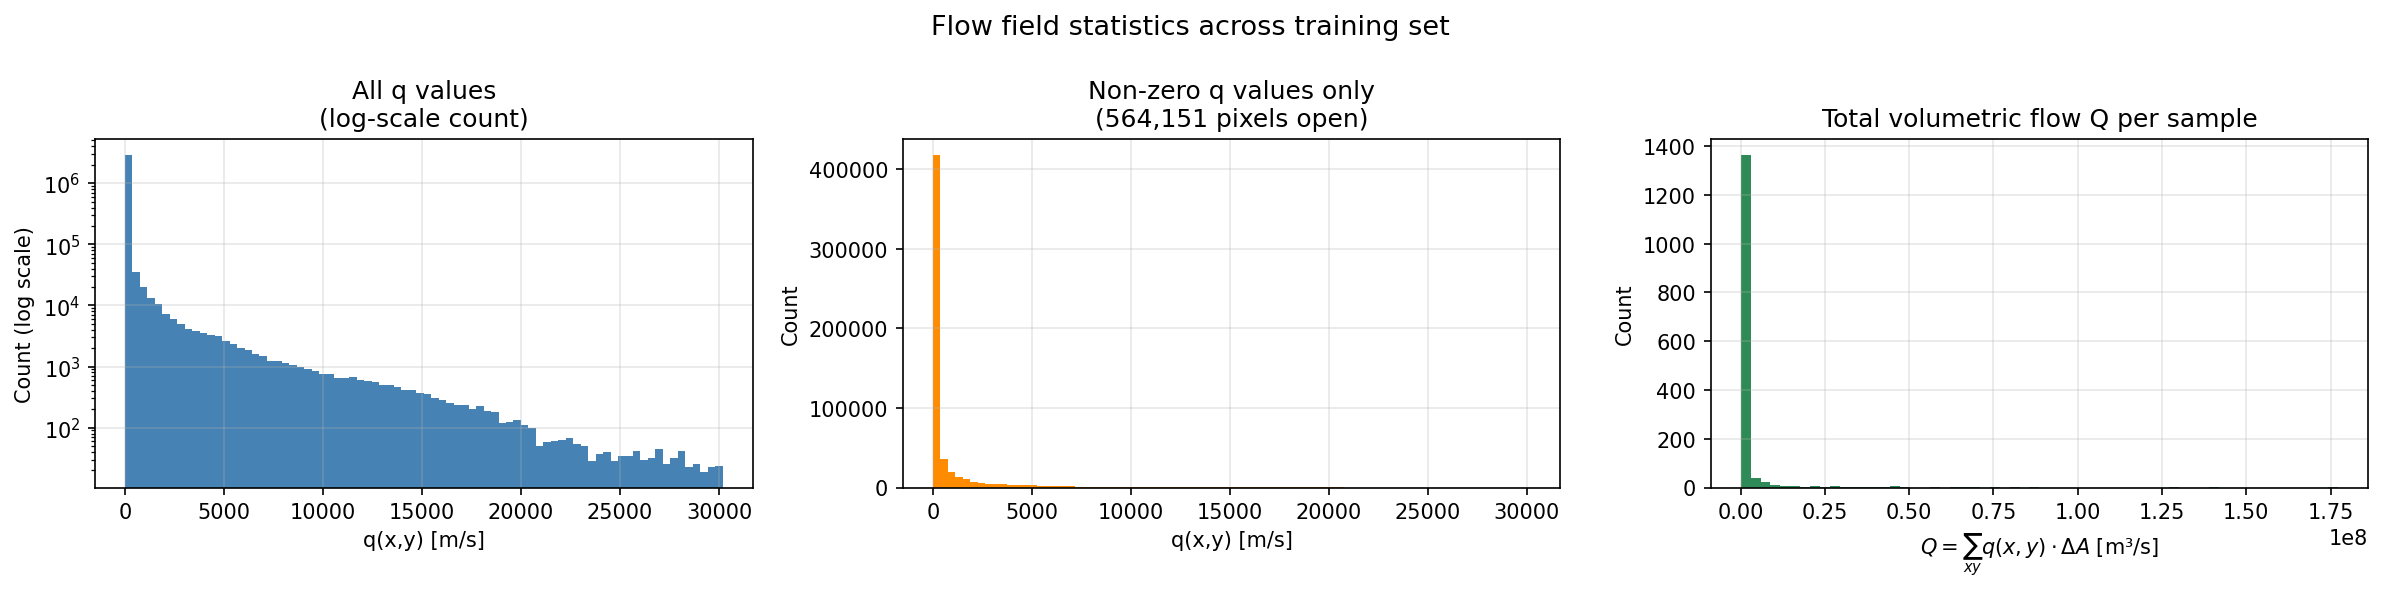
\includegraphics[width=\linewidth]{experiments/plots/exploration_flow_distribution.png}
  \caption{Flow rate statistics across the training set. Left: distribution of all $q(x,y)$ values (log-scale); the large zero-mass at $q=0$ corresponds to closed pixels. Centre: non-zero values only. Right: total volumetric flow $Q = \sum_{xy}q(x,y)\,\Delta A\ [\mathrm{m^3\,s^{-1}}]$ per sample.}
  \label{fig:flow-dist}
\end{figure}

\begin{figure}[h]
  \centering
  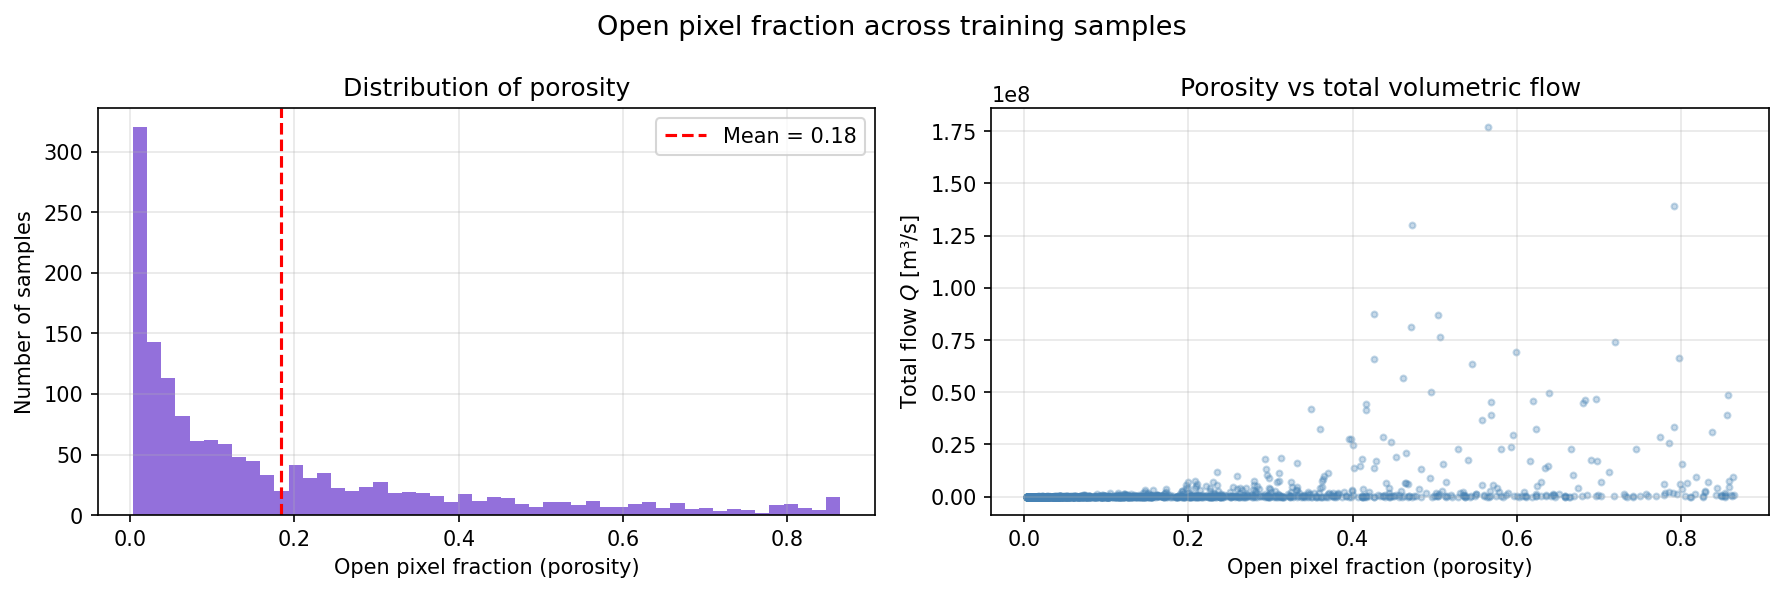
\includegraphics[width=\linewidth]{experiments/plots/exploration_porosity.png}
  \caption{Left: distribution of open pixel fraction (porosity) across training samples; the red dashed line marks the mean. Right: scatter plot of porosity vs total volumetric flow $Q$, illustrating the strong positive correlation.}
  \label{fig:porosity}
\end{figure}

Key observations: (i) the physical parameters span several orders of magnitude, motivating the dimensionless formulation~\eqref{eq:dimless}; (ii) the flow field is identically zero at all closed pixels ($I=0$), a hard physical constraint; (iii) the distribution of $Q$ reflects the wide range of $v_0 = \Delta P\Delta A/(\mu L)$ and porosity in the dataset.

\subsubsection{Loss Functions}

Three loss functions are proposed and evaluated on physical grounds.

\paragraph{L1 -- Kaggle relative error $E$.}
\begin{equation}
  E = \frac{1}{|\mathcal{D}|}\sum_{i\in\mathcal{D}}
      \frac{1}{N_X N_Y}\sum_{x,y}
      \left|\frac{q_i^T(x,y)-q_i(x,y)}{q_i^T(x,y)+\varepsilon}\right|.
  \label{eq:kaggle-loss}
\end{equation}
\textit{Physical assessment.} Dimensionless; $\varepsilon$ prevents division by zero at closed pixels. Each pixel contributes equally in relative terms, which is physically meaningful across the wide range of $v_0$ values. The absolute value makes it non-differentiable at zero residual; $\varepsilon$ introduces an artificial scale below which relative errors are suppressed.

\paragraph{L2 -- Mean squared error (MSE).}
\begin{equation}
  \mathcal{L}_\mathrm{MSE} = \frac{1}{|\mathcal{D}|}\sum_{i}
    \frac{1}{N_X N_Y}\sum_{x,y}
    \bigl[q_i^T(x,y) - q_i(x,y)\bigr]^2.
  \label{eq:mse-loss}
\end{equation}
\textit{Physical assessment.} Dimensions $[\mathrm{m^2\,s^{-2}}]$; not dimensionless. High-velocity pixels dominate the gradient. Under a global rescaling $q\to\lambda q$, the loss scales as $\lambda^2$, violating degree-1 homogeneity and treating different $v_0$ regimes inconsistently. Differentiable everywhere, simple to optimize.

\paragraph{L3 -- Dimensionless relative MSE.}
\begin{equation}
  \mathcal{L}_\mathrm{rel} = \frac{1}{|\mathcal{D}|}\sum_{i}
    \frac{1}{N_X N_Y}\sum_{x,y}
    \left(\frac{q_i^T(x,y) - q_i(x,y)}{q_i^T(x,y)+\varepsilon}\right)^2.
  \label{eq:rel-mse-loss}
\end{equation}
\textit{Physical assessment.} Dimensionless; invariant under $q\to\lambda q$ (degree-0 homogeneous). Differentiable everywhere, unlike $E$, which facilitates gradient-based optimization. Assigns larger relative penalties to outliers than $E$ due to squaring. The $\varepsilon$ caveat applies as in $E$.

\subsubsection{Symmetry-Penalizing Loss}

To quantify and penalize violations of equivariance, define the equivariance residual of a network $f_\theta$ on sample $i$ under transformation $T$ as
\begin{equation}
  r_T^{(i)}(x,y) = f_\theta(T\cdot I_i)(x,y) - T\cdot f_\theta(I_i)(x,y).
  \label{eq:equiv-residual}
\end{equation}
A perfectly equivariant network satisfies $r_T^{(i)}\equiv 0$. The symmetry-penalizing loss is
\begin{equation}
  \mathcal{L}_\mathrm{sym} = \sum_{T\in\mathcal{G}}
    \frac{1}{|\mathcal{D}|}\sum_{i}
    \frac{1}{N_X N_Y}\sum_{x,y}
    \bigl[r_T^{(i)}(x,y)\bigr]^2,
  \label{eq:sym-loss}
\end{equation}
where $\mathcal{G} = \{T_\mathrm{LR},\,T_\mathrm{UD},\,R_{180}\}$. This term can be added to any primary loss as a regularizer:
\begin{equation}
  \mathcal{L}_\mathrm{total} = \mathcal{L}_\mathrm{main} + \alpha\,\mathcal{L}_\mathrm{sym},
  \label{eq:total-loss}
\end{equation}
with $\alpha>0$ a hyperparameter. $\mathcal{L}_\mathrm{sym}$ has units $[\mathrm{m^2\,s^{-2}}]$ (consistent with $\mathcal{L}_\mathrm{MSE}$). When the primary loss is the dimensionless Kaggle error $E$, dimensional consistency requires normalizing: replace $\mathcal{L}_\mathrm{sym}$ with $\mathcal{L}_\mathrm{sym}/v_0^2$ so that both terms are dimensionless and $\alpha$ remains a pure number. $\mathcal{L}_\mathrm{sym}$ also serves as a diagnostic metric to compare models trained with and without hardwired symmetries.

\subsection*{B - Content aligned with point B of the rubric/assignment}

Example of figure, which is referenced as Figure~\ref{fig:example-label}.

\begin{figure}[h]
    \centering
    \includegraphics[width=1\linewidth]{fig/example_image.png}
    \caption{Caption example}
    \label{fig:example-label}
\end{figure}


Example of a subfigure, which elements are referenced as Figure~\ref{fig:first_case} and \ref{fig:full_sub_fig}

\begin{figure}[h]
    \centering
    \subfloat[Subcaption example]{\includegraphics[width=0.49\linewidth]{fig/example_subfig_1.png}%
    \label{fig:first_case}}
    \hfil
    \subfloat[Subcaption example]{\includegraphics[width=0.49\linewidth]{fig/example_subfig_2.png}%
    \label{fig:second_case}}
    \caption{Full caption example.}
    \label{fig:full_sub_fig}
\end{figure}

Alternatively display the same figures spanning across the two text columns as in Figure~\ref{fig:full_sub_fig_alt}

\begin{figure*}[h]
    \centering
    \subfloat[Subcaption example]{\includegraphics[width=0.49\linewidth]{fig/example_subfig_1.png}%
    \label{fig:first_case_alt}}
    \hfil
    \subfloat[Subcaption example]{\includegraphics[width=0.49\linewidth]{fig/example_subfig_2.png}%
    \label{fig:second_case_alt}}
    \caption{Full caption example.}
    \label{fig:full_sub_fig_alt}
\end{figure*}

Bibliography references use instead the \texttt{\\cite} keyword, e.g. \cite{IEEEhowto:kopka}.

\section{Part 2 - Implementation and code}

Discuss key design choices... include key code snippets with \texttt{lstlisting}.
\begin{lstlisting}[language=Python]
import numpy as np
    
def incmatrix(genl1,genl2):
    m = len(genl1)
    n = len(genl2)
    M = None #to become the incidence matrix
    VT = np.zeros((n*m,1), int)  #dummy variable
    
    #compute the bitwise xor matrix
    M1 = bitxormatrix(genl1)
    M2 = np.triu(bitxormatrix(genl2),1) 

    for i in range(m-1):
        for j in range(i+1, m):
            [r,c] = np.where(M2 == M1[i,j])
            for k in range(len(r)):
                VT[(i)*n + r[k]] = 1;
                VT[(i)*n + c[k]] = 1;
                VT[(j)*n + r[k]] = 1;
                VT[(j)*n + c[k]] = 1;
                
                if M is None:
                    M = np.copy(VT)
                else:
                    M = np.concatenate((M, VT), 1)
                
                VT = np.zeros((n*m,1), int)
    
    return M
\end{lstlisting}

Showcase convergence/absence of overfit...





\section{Conclusion}
Always sum up your message and results in a concluding section.


% references section

% can use a bibliography generated by BibTeX as a .bbl file
% BibTeX documentation can be easily obtained at:
% http://mirror.ctan.org/biblio/bibtex/contrib/doc/
% The IEEEtran BibTeX style support page is at:
% http://www.michaelshell.org/tex/ieeetran/bibtex/
%\bibliographystyle{IEEEtran}
% argument is your BibTeX string definitions and bibliography database(s)
%\bibliography{IEEEabrv,../bib/paper}
%
% <OR> manually copy in the resultant .bbl file
% set second argument of \begin to the number of references
% (used to reserve space for the reference number labels box)
\begin{thebibliography}{1}

\bibitem{IEEEhowto:kopka}
H.~Kopka and P.~W. Daly, \emph{A Guide to \LaTeX}, 3rd~ed.\hskip 1em plus
  0.5em minus 0.4em\relax Harlow, England: Addison-Wesley, 1999.

\end{thebibliography}

\begin{appendices}
\section{Appendix A title}
The contents...

\end{appendices}



% that's all folks
\end{document}


